The 

% Duplication
In practice this happens through a replication of the previous layer, where
the output from the previous layer feeds into to both parallel 
layers ($e$ and $e'$).
In the other end, the two layers are merged such that each output neuron
is represented individually in a population with the size $e + e'$.
By not entangling the output dimensions, the following layers can choose
to ignore parts of the input, irrespective of the other parallel layer.
This parallelisation represents the duplication that occurs
in neural circuits, where structurally similar sub-networks, that are
fed the same stimuli, appear to contribute with semantically different
information (see \ref{sec:ref}).

% An optimal approach would be to find a tool that leverages the similarities
% of the network types, while integrating with the diverse simulated or emulated
% targets.
% That is, an abstract model of neural networks that can translate into
% heterogeneous back-ends, while retaining a high degree of inter-model validity.

% A domain-specific language (DSL) called Volr was recently presented to
% construct reproducible \gls{NN} experiments
% \autocite{Pedersen2018:volr}.

% Some work was required to fully support learning mechanisms on
% neuromorphic hardware, and the DSL, as well as the tooling around it, has been
% extended for the purpose of this thesis (see appendix \ref{appendix:volr})
% The following section describes the grammar and anatomy of Volr in detail.

% In practice a network is built by describing a graph.
% The nodes in the graph consist of \texttt{populations} of neurons and the edges
% are connection-set matrices to other populations \autocite{Djurfeldt2012}.
% % TODO: Describe CSA
% \texttt{Populations} can consist of any positive number of neurons and is
% required to have at least one connection.
% Connections can be recursive, resulting in a potentially cyclic graph.
% Both the connections and the \texttt{populations} can be annotated with features
% such as connection weight and neuron parameters (see \nameref{appendix:volr}).
% The parameters are treated differently depending on the experiment target (see
% sections \ref{sec:volr-NEST} and \ref{sec:volr-BrainScaleS}).

% \subsubsection{Experiment targets}
% The final element in a Volr experiment is its targets.
% A target describe a destination environments on which to run the experiment.
% These are described in detail in section \ref{sec:volr-targets}, and are
% referenced in the grammar as simple strings.

% \subsection{Volr semantics}


% \section{Neural network simulation targets in Volr} \label{sec:volr-targets}

% % TODO :Write how fields are interpreted
% % TODO: Write how input is interpreted

% Volr exploits the structural similarities between \gls{ANN} and \gls{SNN} to
% translate the model to both spiking and artificial network platforms (back-ends).

% In the remainder of the chapter the three emulation back-ends, shown in figure
% \ref{fig:volr}, are described:
% a machine learning target for \gls{ANN}s and a neuron simulation target, as well
% as a neuromorphic hardware target, for \gls{SNN}s.

% \begin{figure}
%   \centering
%   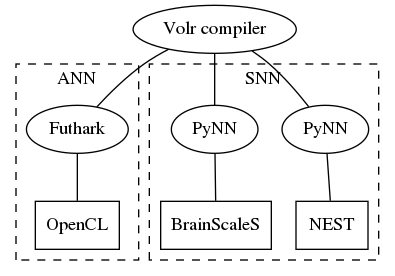
\includegraphics[width=0.6\textwidth]{images/volr-architecture.png}
%   \caption{The translation from the Volr DSL to \gls{ANN} simulations in OpenCL via
%     \gls{Futhark} and to \gls{SNN} simulations on \gls{NEST} and \gls{BrainScaleS}
%     via the \gls{Myelin} middleware.
%   }
%   \label{fig:volr}
% \end{figure}

% \subsection{Translation to Futhark} \label{sec:volr-futhark}
% Futhark is a functional data-parallel programming language \autocite{Henriksen2017}.
% It offers a number of compilation targets such as \gls{OpenCL}, which is
% particularly interesting for this thesis because of its capacity for hardware
% acceleration.

% The practical translation from the Volr model to Futhark is built on recurrent
% \gls{ANN} with stochastic gradient descent backpropagation
% \autocite{russel2007, schmidhuber2014}.
% Each neuron population is considered as a single layer, whose connections are
% determined by a connection matrix.

% % Deal with recurrent connections
% % Describe how this relates to layers

% ... To be continued ...

% \subsection{Spiking neural network simulations via PyNN} \label{sec:volr-pynn}
% The Python neural network simulation interface PyNN is designed as a
% "simulator-independent language for building neuronal network models"
% \autocite{PyNN2018}.
% It aims to reduce the problem of diverse, and occasionally unique, descriptions
% of neural network experiments for different simulation back-ends \autocite{Davison2009}.
% PyNN has been adapted by a number of simulators, including the NEST simulation
% platform and the neuromorphic BrainScaleS wafer system
% \autocite{Davison2009, Helias2012, Schmitt2017}.

% There are still simulator-dependent configurations that seems unlikely to be
% adopted into PyNN in the immediate future\footnote{
%   Particularly hardware mapping configurations are hard to abstract in a general
%   interface.
% }.
% For that reason Volr provides simulation-specific PyNN scripts that can
% interpret the model in the context of each simulation target.
% A middleware, dubbed \gls{Myelin}, was invented to translate the \gls{NN} model
% into a static intermediate representation in JSON.
% The JSON standard was chosen for the task because of its concise syntax while
% still retaining human readability.

% The advantage of the static experiment representation being, that the experiment
% easily a) transports to the target PyNN scripts without losing any information,
% and b) duplexes between several experiment; the same experiment setup is
% trivial to setup on multiple targets at once.

% The correct execution of the experiments relies on the PyNN scripts to exploit
% the simulator to represent the Volr model as accurately as possible.
% Fortunately PyNN is designed to cover exactly such a use case, so properties
% related to the \gls{NN} models itself (such as network topology and population
% attributes) were faithfully reproduced across the simulators.
% However, the simulators deviate in a number of ways that are relevant to
% mention.
% The following two sections explains the steps necessary to achieve accurate
% experiment environments in \gls{NEST} and \gls{BrainScaleS}.

% \subsubsection{Translation to PyNN} \label{sec:volr-translation}

% \subsubsection{Translation to NEST} \label{sec:volr-NEST}
% ... To be continued ...
% \subsubsection{Translation to BrainScaleS} \label{sec:volr-BrainScaleS}
% ... To be continued ...
\label{ref:Cairo}
